\documentclass[12pt,twoside]{article}

\usepackage{weiiszablon}
\usepackage{placeins}
\usepackage{tikz} % Do używania zmiennych przy numerowaniu definicji - można usunąć na samym końcu i ręcznie ponumerować
\usepackage{listings}
\usepackage{amssymb}

\author{Gabriel Lichacz}
\studentID{164174}

\title{Rozpoznawanie rysunków grafów}
\titleEN{Recognition of graphs}

\newcommand{\rodzajPracyNo}{2}

%%% promotor
\supervisor{dr Paweł Bednarz}
\supervisorEN{Paweł Bednarz PhD}

\abstract{Treść streszczenia po polsku}
\abstractEN{Treść streszczenia po angielsku}

\begin{document}

% strona tytułowa
\maketitle

\blankpage

% spis treści
\tableofcontents

\clearpage
\blankpage

\section*{Wykaz symboli}
$G$ - graf

$V(G)$ - zbiór wierzchołków grafu $G$

$E(G)$ - zbiór krawędzi grafu $G$

$C_n$ - cykl $n$-wierzchołkowy

$D$ - digraf

$K_n$ - graf pełny

$N_n$ - graf bezkrawędziowy

$P_n$ - ścieżka $n$-wierzchołkowa

% -- TO DO -- % More
\clearpage

\section{Wstęp}
Graf definiuje się jako pewną parę uporządkowaną $G = (V, E)$, gdzie $V$ zbiór wierzchołków,
a $E$ to zbiór krawędzi, które łączą niektóre z tych wierzchołków.
Takie obiekty mozna przedstawić graficznie jako reprezentację danych,
w której wartości są przedstawione w pewien uporządkowany sposób, zwykle w relacji do siebie nawzajem.
„\textit{Stanowią wygodny aparat do modelowania różnych obiektów, (...) i odpowiednio interpretowane
- mogą zawierać pewne informacje}”\cite{Wloch2008}.

Teoria grafów to dziedzina matematyki zajmująca się badaniem właściwości grafów,
będąca bardzo ważnym narzędziem w wielu „\textit{dziedzinach od rachunku operacyjnego, chemii, po genetykę, lingiwistykę
oraz od elektroniki i geografii po socjologię i architekturę}”\cite{Wilson2012}.
Grafy dają możliwość zobrazowania pewnych modeli, co jest szczególnie korzystne w analizie wzorców.
W kontekście grafów warto podkreślić ich zastosowanie poza teoretycznymi analizami.

W dziedzinach informatycznych, grafy stanowią fundament wielu algorytmów, takich jak algorytmy przeszukiwania,
algorytmy najkrótszej ścieżki, drzew rozpinających, czy modeli sieci.
Przykładem może być tutaj wyszukiwanie najkrótszej trasy, chociażby w nawigacji GPS,
gdzie wierzchołki odpowiadają skrzyżowaniom, a krawędzie drogom.
W przypadku znajdowania najbardziej optymalnych tras, warto wymienić takie algorytmy jak $A*$, Bellmana-Forda czy Dijkstry.

\begin{figure}[ht]
	\centering
	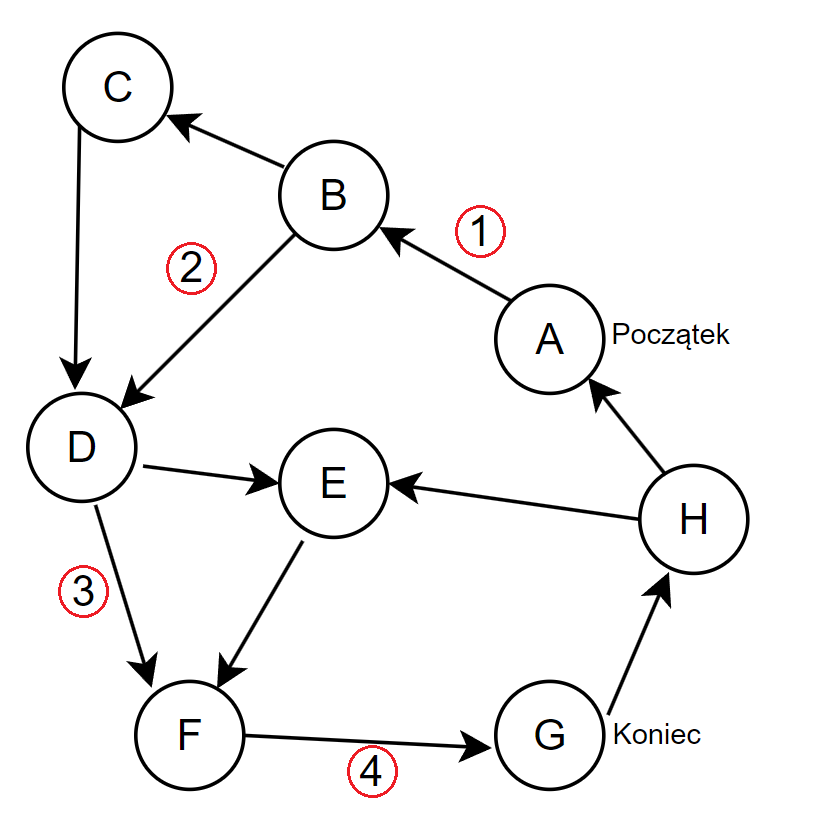
\includegraphics[height=6cm]{partials/images/intro_shortest_path.png}
	\caption{Przykład grafu z wyznaczoną najkrótszą ścieżką od wierzchołka $A$ do $G$}
    \label{Fig:intro-1}
\end{figure}

Duże znaczenie mają również w reprezentacji i modelowaniu struktur danych, takich jak bazy danych.
Najczęściej stosowane bazy danych, tj. relacyjne, zbudowane są w sposób, który grafy mogą doskonale zobrazować -
wierzchołki odpowiadają kolumnom w tabelach a połączenia między nimi to krawędzie, reprezentujące relacje.

\begin{figure}[ht]
	\centering
	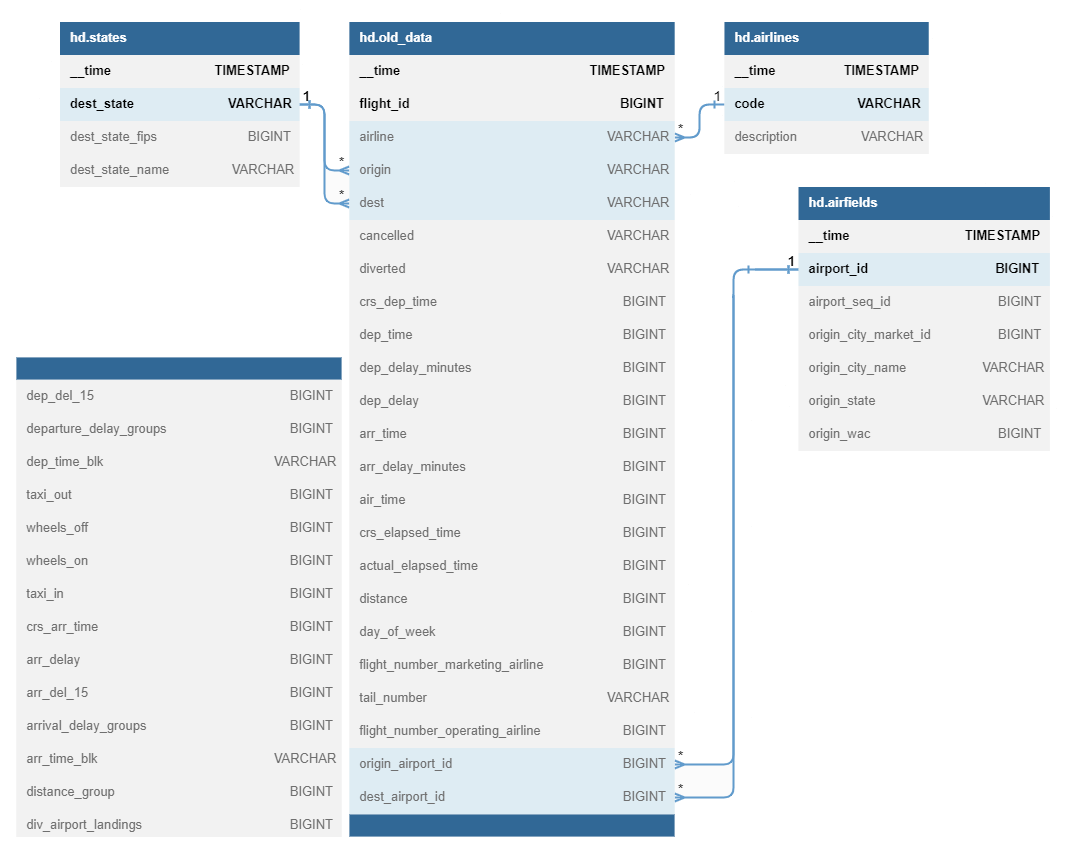
\includegraphics[height=7.5cm]{partials/images/intro_database.png}
	\caption{Przykładowy schemat relacyjnej bazy danych}
    \label{Fig:intro-2}
\end{figure}

W biologii, grafy pełnią ważną rolę w modelowaniu układu nerwowego, sieci białek,
szlaków metabolicznych oraz interakcji między genami.
W genetyce wykorzystuje się je między innymi do analizy drzew filogenetycznych,
co pozwala chociażby na śledzenie relacji ewolucyjnych między organizmami,
z liśćmi reprezentującymi żywe organizmy, a wierzchołkami pośrednimi jako ich wspólnymi przodkami \cite{Erciyes2023}.

\begin{figure}[ht]
	\centering
	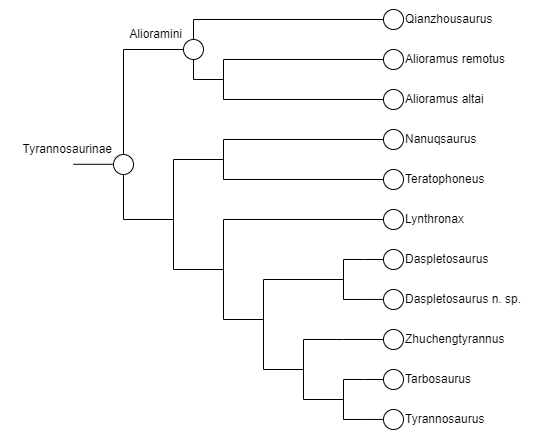
\includegraphics[width=12cm]{partials/images/intro_dino.png}
	\caption{Filogenetyczne relacje Tyrannosaurinae.
		Źródło: opracowanie własne na podstawie: Brusatte, S., Carr, T.
		The phylogeny and evolutionary history of tyrannosauroid dinosaurs, Sci Rep 6, 20252 (2016)}
    \label{Fig:intro-3}
\end{figure}

Natomiast w chemii, grafy służą do reprezentacji struktury molekularnej związków chemicznych,
umożliwiając naukowcom analizę ich właściwości i reaktywności.
Znaczenie teorii grafów dla chemii wynika głównie z istnienia zjawiska izomeryzmu,
które jest uzasadnione przez teorię struktury chemicznej.
Wszystkie wzory strukturalne związków o wiązaniach kowalencyjnych są grafami,
które nazywane są grafami molekularnymi \cite{Balaban1985}.

\begin{figure}[ht]
	\centering
	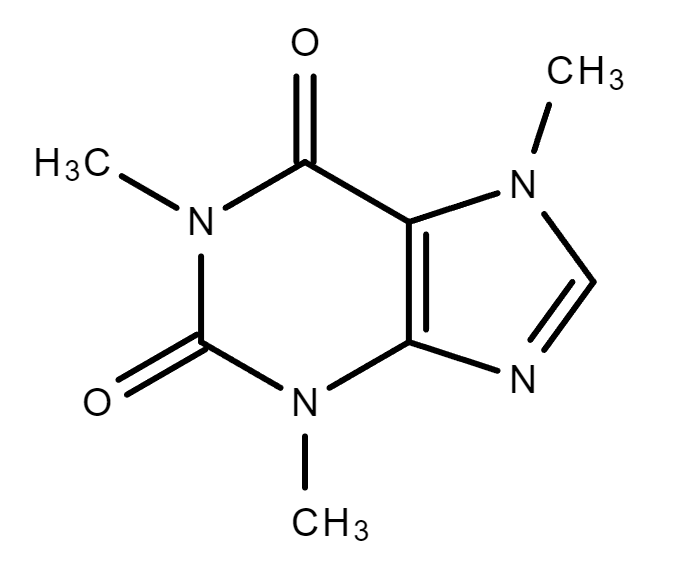
\includegraphics[height=5.5cm]{partials/images/intro_chem.png}
	\caption{Struktura molekularna kofeiny}
    \label{Fig:intro-4}
\end{figure}

W lingwistyce, przy pomocy grafów możliwe jest modelowanie struktury języka, analiza morfologiczna czy syntaktyczna.
Stosowane są również przez wiele innych dziedzin, takich jak gramatyka generatywna,
będąca kandydatem na teoretyczną podstawę biolingwistyki.
Przez ponad pół wieku, wykorzystywała ona notację drzewa jako pomocnicze narzędzie do wyrażania struktur językowych,
lecz takie podejście zostało podważone przez jednego z autorytetów w dziedzinie lingwistyki - Noama Chomsky'ego \cite{Arikawa2019}.
Dzięki grafom, możliwe jest również lepsze zrozumienie i przetwarzanie języka naturalnego przez komputery,
co stanowi podstawę technologii takich jak tłumaczenie automatyczne czy rozpoznawanie mowy.

Teoria grafów znajduje także zastosowanie w analizie sieci społecznych, gdzie pomagają w badaniu relacji między ludźmi.
Wielu psychologów i socjologów zajmuje się tematem struktur wynikających z relacji między różnymi podmiotami.
Przykładami takich zależności mogą być sieci komunikacyjne między ludźmi, relacje dominacji i uległości w grupie,
wpływ lub władza jednych podmiotów nad innymi, czy relacje między różnymi aspektami pola psychologicznego danej osoby lub jej osobowości \cite{Harary1953}.
Bardzo dużym polem jest również analiza mediów społecznościowych, które to wpływają coraz bardziej na przeciętnego człowieka.
Poprzez gromadzenie i analizę danych dotyczących połączeń między użytkownikami, wzorców interakcji i zachowań komunikacyjnych,
analiza mediów społecznościowych pozwala zauważyć pewne struktury społeczne i zidentyfikować wzorce leżące u podstaw interakcji w ich obrębie.
Wszystko to możliwe jest do modelowania za pomocą struktur znanych z teorii grafów \cite{Umami2024}.

\begin{figure}[ht]
	\centering
	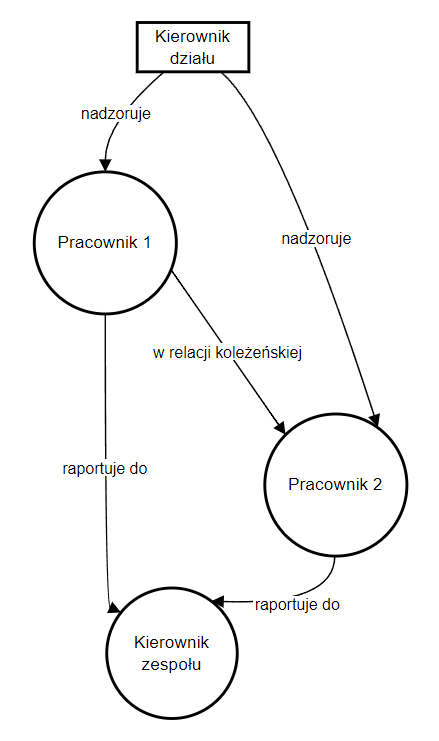
\includegraphics[height=8.5cm]{partials/images/intro_social.png}
	\caption{Przykład sieci relacji pomiędzy pracownikami w dziale danej firmy}
    \label{Fig:intro-5}
\end{figure}

Rozpoznawanie wzorców, nam ludziom, pozwala na szybszą naukę przez rozpoznawanie czegoś, co już wcześniej widzieliśmy.
W bardzo dużym uproszczeniu, algorytmy uczenia maszynowego działają w podobny sposób.
Gdy model zostanie prawidłowo nauczony na pewnych danych,
jest w stanie rozpoznawać podobne wzorce w innych, nigdy wcześniej nie widzianych.

Podsumowując, grafy są niezwykle wszechstronnym narzędziem,
które znajduje zastosowanie w bardzo wielu dziedzinach nauki i technologii.
Ich zdolność do reprezentowania skomplikowanych struktur i relacji w sposób zrozumiały, przystępny i czytelny jest nieoceniona.
Dzięki nim możliwe jest również analizowanie i przetwarzanie informacji w efektywniejszy sposób,
niż informacji nieustrukturyzowanych. 

Celem pracy jest zobrazowanie owej zależności, na przykładzie nauczenia sieci neuronowej,
w taki sposób, by po wytrenowaniu na kilku typach grafów stworzonych sztucznie,
model był w stanie rozpoznać dane wzorce i je nazwać, w przestrzeni rzeczywistej.

\section{Podstawowe definicje teorii grafów}
Praca opiera się na wykorzystaniu języka R oraz Python do generowania zbiorów danych,
wszelkich manipulacji na nich oraz ich klasyfikacji.

\subsection{Język R}

\begin{figure}[ht]
	\centering
	
\includegraphics[height=2cm]{resources/technologies/images/logo_r.png}
	\caption{Logo R \cite{strR}}
	\label{Fig:tech-r}
\end{figure}
\FloatBarrier

Język R~to szeroko stosowany w~statystyce, analizie danych oraz naukach przyrodniczych język interpretowalny.
Nie ma on skomplikowanej składni i jest przystosowany do bycia jak najbardziej przyjaznym dla nowego użytkownika.
Oprócz dużych możliwości obliczeniowych, jest również świetnym narzędziem do wizualizacji danych,
co spowodowało, że został wybrany do stworzenia zbioru danych.
Grafy wygenerowane zostały przy pomocy biblioteki igraph w wersji~2.0.3.
Jest to pakiet do tworzenia i~analizy struktur sieci, a co za tym idzie oferuje bogaty wybór funkcji do
generowania losowych i~regularnych grafów oraz ich wizualizacji.

\subsection{Język Python}

\begin{figure}[ht]
	\centering
	
\includegraphics[height=2cm]{resources/technologies/images/logo_python.png}
	\caption{Logo Python \cite{strPython}}
	\label{Fig:tech-python}
\end{figure}
\FloatBarrier

Język Python jest jednym z najpopularniejszych języków wysokopoziomowych ogólnego przeznaczenia.
Zawdzięcza to swojej wszechstronności oraz prostocie składni.
Znaczna liczba bibliotek pozwala na wykorzystywanie Pythona od
prostych skryptów, przez analizę danych, aż po rozbudowane aplikacje, takie jak całe
systemy największych gigantów technologicznych, np. Google. Język ten jest szeroko
wykorzystywany w dziedzinie Data Science do wizualizacji, analizy~i przetwarzania danych oraz w uczeniu maszynowym.
Ostatnie z wymienionych zastosowań zadecydowało~o wyborze języka Python jako narzędzia do stworzenia modelu klasyfikacji grafów.
Wykorzystana została biblioteka Keras z pakietu Tensorflow.

\subsection{Stanowisko pracy}
Całość pracy, tj. generacja danych, modele oraz testy, została przygotowana na komputerze osobistym o parametrach:

\begin{itemize}[label=-,labelsep=0.4cm,leftmargin=0.6cm]
\item CPU: i5-10400F 2.9 GHz
\item RAM: 32 GB 3200 MHz
\item GPU: ADM Radeon RX 5600 XT 6GB
\item Dysk: 2 x 1 TB HDD, 1 TB NVMe, 120 GB SSD
\item System operacyjny: Windows 10
\end{itemize}
System nie posiada karty graficznej zoptymalizowanej pod zastosowania uczenia maszynowego.
Biblioteki języka Python obsługują jednak karty graficzne AMD, co umożliwia pracę.

\section{Uczenie maszynowe}
Praca opiera się na wykorzystaniu języka R oraz Python do generowania zbiorów danych,
wszelkich manipulacji na nich oraz ich klasyfikacji.

\subsection{Język R}

\begin{figure}[ht]
	\centering
	
\includegraphics[height=2cm]{resources/technologies/images/logo_r.png}
	\caption{Logo R \cite{strR}}
	\label{Fig:tech-r}
\end{figure}
\FloatBarrier

Język R~to szeroko stosowany w~statystyce, analizie danych oraz naukach przyrodniczych język interpretowalny.
Nie ma on skomplikowanej składni i jest przystosowany do bycia jak najbardziej przyjaznym dla nowego użytkownika.
Oprócz dużych możliwości obliczeniowych, jest również świetnym narzędziem do wizualizacji danych,
co spowodowało, że został wybrany do stworzenia zbioru danych.
Grafy wygenerowane zostały przy pomocy biblioteki igraph w wersji~2.0.3.
Jest to pakiet do tworzenia i~analizy struktur sieci, a co za tym idzie oferuje bogaty wybór funkcji do
generowania losowych i~regularnych grafów oraz ich wizualizacji.

\subsection{Język Python}

\begin{figure}[ht]
	\centering
	
\includegraphics[height=2cm]{resources/technologies/images/logo_python.png}
	\caption{Logo Python \cite{strPython}}
	\label{Fig:tech-python}
\end{figure}
\FloatBarrier

Język Python jest jednym z najpopularniejszych języków wysokopoziomowych ogólnego przeznaczenia.
Zawdzięcza to swojej wszechstronności oraz prostocie składni.
Znaczna liczba bibliotek pozwala na wykorzystywanie Pythona od
prostych skryptów, przez analizę danych, aż po rozbudowane aplikacje, takie jak całe
systemy największych gigantów technologicznych, np. Google. Język ten jest szeroko
wykorzystywany w dziedzinie Data Science do wizualizacji, analizy~i przetwarzania danych oraz w uczeniu maszynowym.
Ostatnie z wymienionych zastosowań zadecydowało~o wyborze języka Python jako narzędzia do stworzenia modelu klasyfikacji grafów.
Wykorzystana została biblioteka Keras z pakietu Tensorflow.

\subsection{Stanowisko pracy}
Całość pracy, tj. generacja danych, modele oraz testy, została przygotowana na komputerze osobistym o parametrach:

\begin{itemize}[label=-,labelsep=0.4cm,leftmargin=0.6cm]
\item CPU: i5-10400F 2.9 GHz
\item RAM: 32 GB 3200 MHz
\item GPU: ADM Radeon RX 5600 XT 6GB
\item Dysk: 2 x 1 TB HDD, 1 TB NVMe, 120 GB SSD
\item System operacyjny: Windows 10
\end{itemize}
System nie posiada karty graficznej zoptymalizowanej pod zastosowania uczenia maszynowego.
Biblioteki języka Python obsługują jednak karty graficzne AMD, co umożliwia pracę.

\section{Wykorzystywane technologie}
Praca opiera się na wykorzystaniu języka R oraz Python do generowania zbiorów danych,
wszelkich manipulacji na nich oraz ich klasyfikacji.

\subsection{Język R}

\begin{figure}[ht]
	\centering
	
\includegraphics[height=2cm]{partials/images/logo_r.png}
	\caption{Logo R}
	\label{Fig:tech-r}
\end{figure}
\FloatBarrier

Język R~to szeroko stosowany w~statystyce, analizie danych oraz naukach przyrodniczych język interpretowalny.
Nie ma on skomplikowanej składni i jest przystosowany do bycia jak najbardziej przyjaznym dla nowego użytkownika.
Oprócz dużych możliwości obliczeniowych, jest również świetnym narzędziem do wizualizacji danych,
co spowodowało, że został wybrany do stworzenia zbioru danych.
Grafy wygenerowane zostały przy pomocy biblioteki igraph w wersji~2.0.3.
Jest to pakiet do tworzenia i~analizy struktur sieci, a co za tym idzie oferuje bogaty wybór funkcji do
generowania losowych i~regularnych grafów oraz ich wizualizacji.

\subsection{Język Python}

\begin{figure}[ht]
	\centering
	
\includegraphics[height=2cm]{partials/images/logo_python.png}
	\caption{Logo Python}
	\label{Fig:tech-python}
\end{figure}
\FloatBarrier

Język Python jest jednym z najpopularniejszych języków wysokopoziomowych ogólnego przeznaczenia.
Zawdzięcza to swojej wszechstronności oraz prostocie składni.
Znaczna liczba bibliotek pozwala na wykorzystywanie Pythona od
prostych skryptów, przez analizę danych, aż po rozbudowane aplikacje, takie jak całe
systemy największych gigantów technologicznych, np. Google. Język ten jest szeroko
wykorzystywany w dziedzinie Data Science do wizualizacji, analizy~i przetwarzania danych oraz w uczeniu maszynowym.
Ostatnie z wymienionych zastosowań zadecydowało~o wyborze języka Python jako narzędzia do stworzenia modelu klasyfikacji grafów.
Wykorzystana została biblioteka Keras z pakietu Tensorflow.

\subsection{Stanowisko pracy}
Całość pracy, tj. generacja danych, modele oraz testy, została przygotowana na komputerze osobistym o parametrach:

\begin{itemize}[label=-,labelsep=0.4cm,leftmargin=0.6cm]
\item CPU: i5-10400F 2.9 GHz
\item RAM: 32 GB 3200 MHz
\item GPU: ADM Radeon RX 5600 XT 6GB
\item Dysk: 2 x 1 TB HDD, 1 TB NVMe, 120 GB SSD
\item System operacyjny: Windows 10
\end{itemize}
System nie posiada karty graficznej zoptymalizowanej pod zastosowania uczenia maszynowego.
Biblioteki języka Python obsługują jednak karty graficzne AMD, co umożliwia pracę.

\section{Testy}
Praca opiera się na wykorzystaniu języka R oraz Python do generowania zbiorów danych,
wszelkich manipulacji na nich oraz ich klasyfikacji.

\subsection{Język R}

\begin{figure}[ht]
	\centering
	
\includegraphics[height=2cm]{resources/technologies/images/logo_r.png}
	\caption{Logo R \cite{strR}}
	\label{Fig:tech-r}
\end{figure}
\FloatBarrier

Język R~to szeroko stosowany w~statystyce, analizie danych oraz naukach przyrodniczych język interpretowalny.
Nie ma on skomplikowanej składni i jest przystosowany do bycia jak najbardziej przyjaznym dla nowego użytkownika.
Oprócz dużych możliwości obliczeniowych, jest również świetnym narzędziem do wizualizacji danych,
co spowodowało, że został wybrany do stworzenia zbioru danych.
Grafy wygenerowane zostały przy pomocy biblioteki igraph w wersji~2.0.3.
Jest to pakiet do tworzenia i~analizy struktur sieci, a co za tym idzie oferuje bogaty wybór funkcji do
generowania losowych i~regularnych grafów oraz ich wizualizacji.

\subsection{Język Python}

\begin{figure}[ht]
	\centering
	
\includegraphics[height=2cm]{resources/technologies/images/logo_python.png}
	\caption{Logo Python \cite{strPython}}
	\label{Fig:tech-python}
\end{figure}
\FloatBarrier

Język Python jest jednym z najpopularniejszych języków wysokopoziomowych ogólnego przeznaczenia.
Zawdzięcza to swojej wszechstronności oraz prostocie składni.
Znaczna liczba bibliotek pozwala na wykorzystywanie Pythona od
prostych skryptów, przez analizę danych, aż po rozbudowane aplikacje, takie jak całe
systemy największych gigantów technologicznych, np. Google. Język ten jest szeroko
wykorzystywany w dziedzinie Data Science do wizualizacji, analizy~i przetwarzania danych oraz w uczeniu maszynowym.
Ostatnie z wymienionych zastosowań zadecydowało~o wyborze języka Python jako narzędzia do stworzenia modelu klasyfikacji grafów.
Wykorzystana została biblioteka Keras z pakietu Tensorflow.

\subsection{Stanowisko pracy}
Całość pracy, tj. generacja danych, modele oraz testy, została przygotowana na komputerze osobistym o parametrach:

\begin{itemize}[label=-,labelsep=0.4cm,leftmargin=0.6cm]
\item CPU: i5-10400F 2.9 GHz
\item RAM: 32 GB 3200 MHz
\item GPU: ADM Radeon RX 5600 XT 6GB
\item Dysk: 2 x 1 TB HDD, 1 TB NVMe, 120 GB SSD
\item System operacyjny: Windows 10
\end{itemize}
System nie posiada karty graficznej zoptymalizowanej pod zastosowania uczenia maszynowego.
Biblioteki języka Python obsługują jednak karty graficzne AMD, co umożliwia pracę.

\section{Podsumowanie i wnioski końcowe}
Celem pracy było zbudowanie modeli sztucznych sieci neuronowych,
które byłby w stanie rozpoznawać wybrane pięć typów grafów.
Wykorzystany w tym celu został język R, wraz z jego bibliotekami, do wytworzenia danych wejściowych modeli
oraz język Python, z~pakietem Tensorflow, do zaprojektowania i~przetestowania modeli.
Praca pokazała, że możliwe jest stworzenie modelu, który rozpozna rysowane odręcznie rysunki grafów
z pewnością lepszą niż wybór losowy.
Najlepszy model osiągnął realną dokładność wynoszącą 45\%,
co wciąż pozostawia pewne pole do rozwoju owego modelu.

Praca zarysowuje temat grafów oraz ich podstawowych pojęć,
a także wykorzystania teorii grafów w różnych dziedzinach nauki.
Przedstawiona jest również idea uczenia maszynowego,
jego rodzaje oraz sam proces działania.
W pracy przedstawiono proces tworzenia zbioru danych za pomocą skryptów R,
oraz kolejne kroki budowy modeli sztucznych sieci neuronowych do rozpoznawania grafów.
Przeprowadzono analizę ich skuteczności zarówno na danych syntetycznych, jak i~rzeczywistych.
Sieci neuronowe były trenowane na wygenerowanych rysunkach grafów,
co umożliwiło stworzenie modeli do klasyfikacji grafów zewnętrznych.
Następnie modele te przetestowano na rzeczywistych rysunkach grafów,
aby zweryfikować ich praktyczną użyteczność oraz ocenić,
w jakim stopniu ich teoretyczna dokładność przekłada się na realne zastosowania.

W testach zastosowano naukę na maksymalnie 75 epokach.
Analizując krzywe dokładności i~straty modeli, można dojść do wniosku,
że dłuższe uczenie nie przyniosłoby pozytywnych skutków lub znikome pozytywne.
Przeprowadzono również testy na mniejszych liczbach epok, lecz wartości takie jak 10, czy 20,
są za małe, by poprawnie nauczyć większość modeli.
Modele osiągały dość wysokie dokładności już po kilku pierwszych epokach,
ale zdecydowana większość z~nich, z~biegiem kolejnych epok, nabierała jeszcze lepszej dokładności.
W przypadku jednego modelu, konieczne było zmniejszenie liczby epok do 55,
ze względu na powstające problemy z~procesem nauczania, po owej epoce.

Uczenie modeli z~wykorzystaniem stałej liczby wierzchołków grafów okazało się bardziej skuteczne
niż nauka na rysunkach grafów o~zmiennej liczbie wierzchołków.

Skomplikowaność modelu i~zastosowane techniki optymalizacyjne rzadko przekładały się na zwiększoną realną dokładność modelu.

W przypadku uczenia najbardziej zmodyfikowanych modeli, to grafy pełne najczęściej dominowały cały zbiór danych,
przez co modele te testach na danych zewnętrznych,
klasyfikowały większość testowych grafów rysowanych odręcznie jako właśnie grafy pełne.

Wyniki eksperymentów pokazały, że modele miewają problemy z przeuczeniem,
ale w przypadku części modeli osiągnięta wysoka dokładność na zbiorach treningowych i walidacyjnych,
przełożyła się na dobre wyniki klasyfikacji danych zewnętrznych.

%%%%%%%%%%%%%% % -- TO DO -- %
Pomimo ogólnie dobrych wyników,
zaobserwowano drobne różnice pomiędzy wynikami na danych syntetycznych i~rzeczywistych,
co sugeruje, że dalsze badania mogą skupić się na udoskonaleniu procesu generowania grafów
lub wprowadzeniu dodatkowych mechanizmów regularyzacyjnych w~celu poprawy zdolności generalizacji modeli.
Przedstawione w~referacie badania wskazują na wysoki potencjał sztucznych sieci neuronowych
w zadaniach związanych z~analizą i~klasyfikacją grafów,
co otwiera nowe możliwości w~kontekście przetwarzania danych graficznych w~praktycznych zastosowaniach.

\clearpage

\section*{Załączniki}
\addcontentsline{toc}{chapter}{Załączniki}

\begin{itemize}[label=-,labelsep=0.4cm,leftmargin=0.6cm]
    \item Skrypt generujący obrazy grafów
    \item Skrypty testowe z~modelem podstawowym
    \item Skrypty testowe z~modelem, z~walidacją krzyżową
    \item Skrypty testowe z~modelem dostosowanym do~nauki grafów o~różnej liczbie wierzchołków
    \item Skrypty testowe z~modelem, z~walidacją krzyżową, dostosowanym do~nauki grafów o~różnej liczbie wierzchołków
    \item Zbiór zewnętrznych grafów testowych
\end{itemize}

\vspace*{\fill}

Wersja online dokumentu, dane oraz kod źródłowy w~języku Python i~R dostępne na~stronie:
https://github.com/gabriellichacz/graph\_classification

\clearpage

\addcontentsline{toc}{section}{Literatura}

\begin{thebibliography}{4}
    \bibitem{Arikawa2019} Arikawa K.: \textit{Graph Theory Teaches Us Something About Grammaticality}. The Prague Bulletin of Mathematical Linguistics No. 112, 2019, pp. 55-82.
    \bibitem{Balaban1985} Balaban A.T.: \textit{Applications of Graph Theory in Chemistry}. Department of Organic Chemistry, Polytefhnic Institute. 76206 Bucharest, Roumania, 1985.
    \bibitem{Brusatte2021} Brusatte, S., Carr, T.: \textit{The phylogeny and evolutionary history of tyrannosauroid dinosaurs}. Sci Rep 6, 20252 (2016). https://doi.org/10.1038/srep20252.
    \bibitem{Chung2021} Chung M.K.: \textit{Graph Theory in Brain Networks}, University of Wisconsin-Madison, 2021.
    \bibitem{Erciyes2023} Erciyes K.: \textit{Graph-Theoretical Analysis of Biological Networks: A Survey}. Computation 2023, 11, 188, DOI: https://doi.org/10.3390/computation11100188.
    \bibitem{Fenner2020} Fenner M.E.: \textit{Uczenie maszynowe w Pythonie dla każdego}. Helion SA, Gliwice 2020.
    \bibitem{Geron2020} Géron A.: \textit{Uczenie maszynowe z użyciem Scikit-Learn i TensorFlow}. Helion SA, Gliwice 2020.
    \bibitem{Goodfellow2016} Goodfellow I., Bengio Y., Courville A.: \textit{Deep Learning}, MIT Press 2016.
    \bibitem{Harary1953} Harary F., Norman R.Z.: \textit{Graph Theory as a Mathematical Model in Social Science}, Research Center for Group Dynamics, University of Michigan, 1953.
    \bibitem{Rodak2021} Rodak K., Kokot I., Kratz E.W.: \textit{Caffeine as a Factor Influencing the Functioning of the Human Body-Friend or Foe?} Nutrients. 2021 Sep 2;13(9):3088.
    \bibitem{Seenappa} Seenappa M.G.: \textit{Graph Classification using Machine Learning Algorithms}. Master's Projects. 725, San Jose State University 2019, DOI: https://doi.org/10.31979/etd.b9pm-wpng.
    \bibitem{Umami2024} Umami M.H., Prihandini R.M., Agatha A.B.: \textit{Application of Graph Theory to Social Network Analysis}, Department of Mathematics Educations, University of Jember, Jember, Indonesia, 2024.
    \bibitem{vanDerMaaten} L.J.P. van der Maaten, Hinton G.E.: \textit{Visualizing High-Dimensional Data Using t-SNE}. Journal of Machine Learning Research 9(Nov):2579-2605, 2008.
    \bibitem{Wilson2012} Wilson R.J.: \textit{Wprowadzenie do teorii grafów}. PWN, Warszawa 2012.
    \bibitem{Wloch2008} Włoch A., Włoch I.: \textit{Matematyka dyskretna. Podstawowe metody i algorytmy teorii grafów}. Oficyna Wydawnicza Politechniki Rzeszowskiej, Rzeszów 2008.
    \bibitem{Wojciechwoski2013} Wojciechowski J., Pieńkosz K.: \textit{Grafy i sieci}. PWN, Warszawa 2013.
    % - TO DO -- % Sprawdzić wywołania
    \bibitem{str3} https://www.kaggle.com/datasets/robikscube/flight-delay-dataset-20182022. Dostęp 06.01.2024.
    \bibitem{str3} https://cran.r-project.org/web/packages/igraph/index.html. Dostęp 10.03.2024.
    \bibitem{str5} https://developers.google.com/machine-learning. Dostęp 20.07.2024.
    \bibitem{str4} https://www.ibm.com/topics. Dostęp 20.07.2024.
    \bibitem{strPython} https://www.python.org/. Dostęp 07.08.2024.
    \bibitem{strR} https://www.r-project.org/. Dostęp 07.08.2024.
    \bibitem{str1} http://student.krk.pl/026-Ciosek-Grybow/rodzaje.html. Dostęp 26.03.2024.
    \bibitem{str6} https://www.tensorflow.org/api\_docs. Dostęp 21.07.2024.
    \bibitem{str2} http://wms.mat.agh.edu.pl/\texttildelow md/ang-pol.pdf. Dostęp 29.03.2024.
\end{thebibliography}

\clearpage

\makesummary

\end{document}